\chapter{State-of-the-Art} \label{chap:sota}

\section*{}

In this chapter we will begin by making a more in depth presentation of the
process of gene expression. This will be followed by a literature and state of
the art review in the fields of genome/\trans{} assembly and data mining.
Lastly, we will present some of the tools used in each of those areas, as well
as some relevant data representation formats for genetic data.

\section{Introduction}

Before dwelling in the details of the state of the art that are on the
foundation of this thesis, it is important to explain some concepts of the
domain of molecular biology. As explained in Section \ref{sec:context}, gene
expression is the mechanism by which an organism's \dna{} can be expressed into
functional genetic products, like proteins, rRNA and tRNA. This process starts
with the genetic code, or nucleotide sequence, of each gene. Different genes in
an organism's \dna{} are responsible for the creation of different genetic
products. The process of gene expression itself is composed by two main stages,
transcription and translation \cite{leic:gene_expr}.

Transcription is the stage at which genetic data in the form of \dna{} is used
to synthesize \rna{}, being this the process that concerns the thesis main
question. Several different types of \rna{} are produced by this process,
including mRNA (which specifies the sequences of amino acids that form a
protein), rRNA and tRNA, both later used in the translation stage. Simplifying a
gene's structure, it can be seen as composed by two types of areas, introns and
exons, as seen in Figure \ref{fig:intron_exon}.

\begin{figure}[!htb]
  \begin{center}
    \leavevmode
    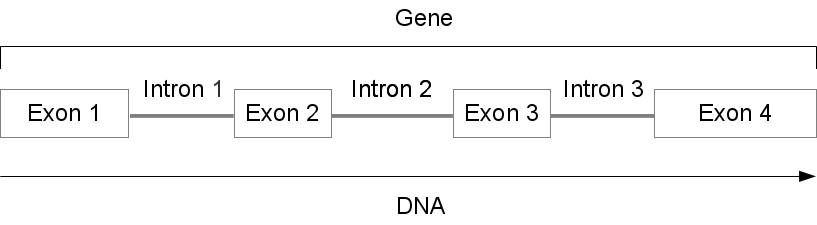
\includegraphics[width=0.7\textwidth]{intron_exon}
    \caption{Overall structure of a gene, with its different areas (simplified)}
    \label{fig:intron_exon}
  \end{center}
\end{figure}

Only the exons are useful in the gene expression process, being also known as
coding regions. Introns, on the other hand, are not used in the process. They
are present in an early stage mRNA molecule, the precursor RNA, but are later
removed (or spliced) in the final molecule before the translation stage
\cite{leic:gene_expr}. Figure \ref{fig:splicing} illustrates the removal of
introns from the mRNA molecule, during the  splicing process. As stated before,
the main goal of this thesis is to explain how the final nucleotide sequence of
each exon affects the transcription speed of the exon itself.

\begin{figure}[!htb]
  \begin{center}
    \leavevmode
    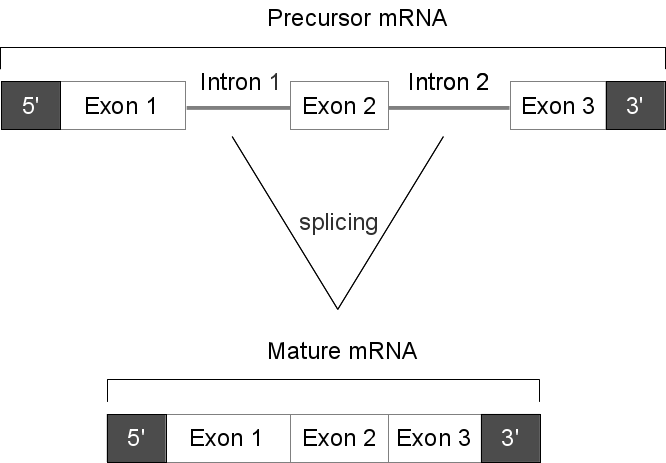
\includegraphics[width=0.58\textwidth]{splicing}
    \caption{The removal (splicing) of introns from the precursor mRNA, during
    the transcription process}
    \label{fig:splicing}
  \end{center}
\end{figure}

After the conclusion of the transcription process comes the translation process.
In this process, the synthesized mRNA is used to specify the sequence of amino
acids that constitute the particular protein being produced. The other types of
RNA molecules (rRNA and tRNA) are also used in this stage of the gene expression
process.

Obtaining this genetic information is done experimentally, by employing a genome
sequencing technique. For quite some time this process was carried out using the
Sanger sequencing method and other similar methods \cite{Reis-Filho2009}. Though
effective, such methods we're notably slow and costly, with large projects like
the Human Genome Project (HGP) consuming roughly thirteen years and US\$ 3
billion. The past few years have seen the appearance and rise in popularity of
the \ngs{} techniques. These techniques differ from the more classical ones by
producing larger amounts of information, in less time. They are also typically
more cost effective than previous techniques, which has greatly contributed to
their popularity. As a disadvantage, \ngs{} techniques produce shorter reads
than their older counterparts, posing a complicated problem in terms of genome
assembly and raising new computational challenges. Although this thesis will not
deal with the problems of sequencing techniques, it is important to indicate
that the read dataset that will be used is a result of \ngs{} techniques. As
such, we will use assembly techniques more suited to situations where short
reads are available.

\section{Genome Assembly and \rnaseq}\label{sec:assembly}

- talk about genome assembly, talk briefly about micro arrays, more about RNA
  seq and de novo vs guided assembly/alignment;\\

\subsection{\rnaseq{} Tools}\label{sec:seqtools}

\subsection{Relevant Standard File Formats}\label{sec:formats}

\subsection{FASTA}

\subsection{FASTQ}

\subsection{SAM and BAM}

\subsection{VCF}

\subsection{GTF and GFF}

\section{Data Mining}\label{sec:mlearning}

\subsection{Data Mining Algorithms}\label{sec:minalgo}

\subsection{Data Mining Tools}\label{sec:mintools}

Except in rare cases of very specific problems, it typically makes no sense for
someone to implement any data mining algorithm that they might need. In fact,
today we have lots of data mining tools (many of which are free), that already
implement many of those algorithms. These tools are usually customizable, making
it easy to adapt them to most problems. Below we'll briefly review some of the
most popular data mining tools, that apply to the specific needs of this thesis.

\subsubsection{RapidMiner}

RapidMiner\footnote{\url{http://www.rapidminer.com/}} is a complete solution for
data mining problems. It's available as a standalone GUI based application, as
seen in Figure \ref{fig:rapidminer}. It is a commercial application, although
its core and earlier versions are distributed under an open source license and
it offers a free version, beyond its multiple paid versions. Being one of the
most popular data mining tools used today, its applications span several
domains, including education, training, industrial and personal applications,
among others. Its functionality can also be easily extended through the use of
plugins\footnote{Plugin is a software module that adds new functionality to an
existing software application. Plugins are typically dependent on the platform
they extend and can't be used as standalone tools.}, reflecting in an increased
value for this tool. One such example in the area of bioinformatics is the
integration plugin between RapidMiner and the
Taverna\footnote{\url{http://www.taverna.org.uk/}} open source workflow
management system \cite{Jupp2011}.

\begin{figure}[!htb]
  \begin{center}
    \leavevmode
    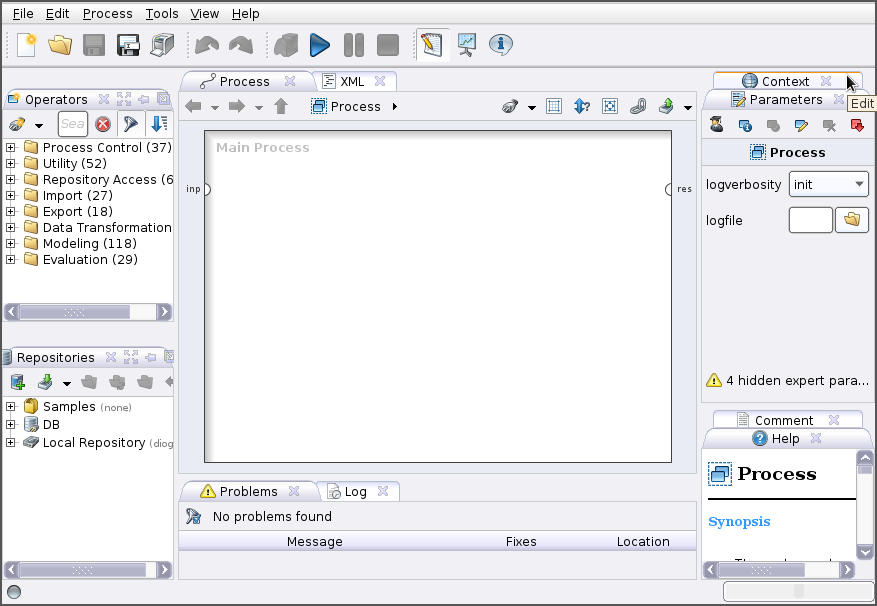
\includegraphics[width=1.0\textwidth]{rapidminer}
    \caption{RapidMiner user interface}
    \label{fig:rapidminer}
  \end{center}
\end{figure}

\subsubsection{Weka}

Weka\footnote{\url{http://www.cs.waikato.ac.nz/ml/weka/}} is an open source tool that
collects several machine learning algorithms and allows its user to easily apply
those algorithms to data mining tasks \cite{Hall}. Created at the University of
Waikato, New Zeland in 1997 (the current version was completely rewritten in
1997, despite the first iteration of the tool being developed as early as 1993),
it's still in active development to date. Weka supports several common data
mining tasks, like data preprocessing, classification, clustering, regression
and data visualization. It's core libraries are written in Java and allow for an
easy integration of its data mining algorithms in pre existing code and
applications. Other than that, Weka can be used directly through a command
line/terminal or through one of its multiple GUI's (Figure \ref{fig:weka}). Its
simple API and well structure architecture allow it to be easily extended by
users, should they need new functionalities.

\begin{figure}[!htb]
  \begin{center}
    \leavevmode
    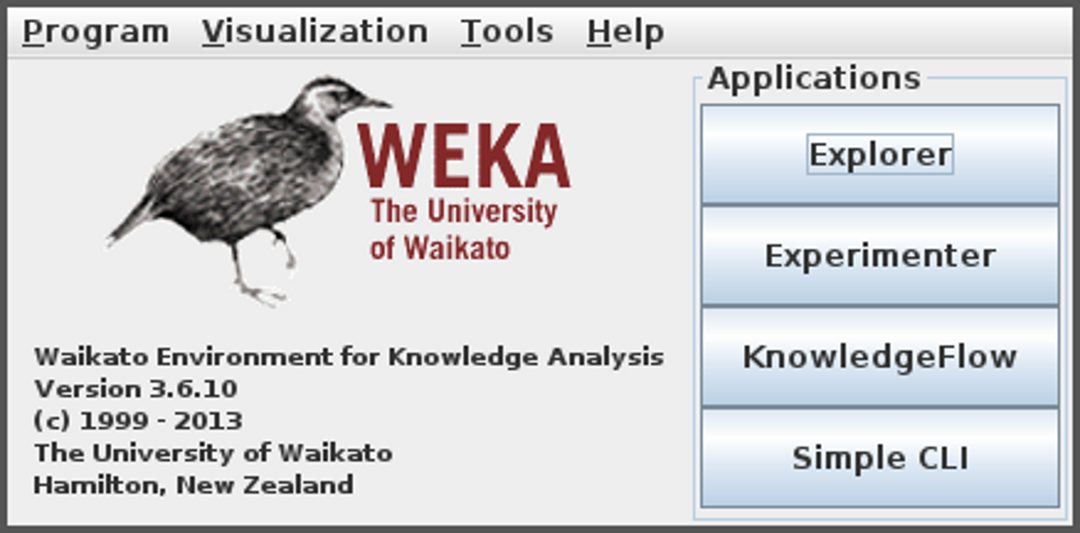
\includegraphics[width=0.7\textwidth]{weka}
    \caption{Weka interface selection}
    \label{fig:weka}
  \end{center}
\end{figure}

\subsubsection{R Language}

R\footnote{\url{http://www.r-project.org/}} is a free programming language and
software environment for statistical computing and graphics generation.
Originally developed by Ross Ihaka and Robert Gentleman at the University of
Auckland, New Zealand in 1993 \cite{Ihaka1998}, it's still under active
development. R is typically used by statisticians and data miners, either for
direct data analysis or for developing new statistical software \cite{Fox2005}.

R is an implementation of the S programming language\footnote{S is an object
oriented statistical programming language, appearing in 1976 at Bell
Laboratories.}, borrowing some characteristics from the Scheme programming
language. It's core is written in a combination of C, Fortran and R itself. It
is possible directly manipulate R objects in languages like C, C++ and Java. R
can be used directly through the command line or through several third party
graphical user interfaces like
Deducer\footnote{\url{http://www.deducer.org/pmwiki/index.php}}. There are also
R wrappers for several scripting languages.

R provides several different statistical and graphical techniques, including
linear and nonlinear modeling, classical statistical tests, time-series
analysis, classification, clustering, among others. It can also be used to
produce publication-quality static graphics. Tools like Sweave
\cite{lmucs-papers:Leisch:2002} allow users to embed R code in \LaTeX{}
documents, for complete data analysis.

\subsubsection*{Bioconductor Package}

Bioconductor is a free and open source set of tools for genomic data analysis,
in the context of molecular biology \cite{lmucs-papers:Leisch:2002}. It is
primarily based on R. It is under active development, with two stable releases
each year. Counting with more than seven hundred different packages, it's the
most comprehensive set of genomic data analysis tools available for the R
programming language. It also provides a set of tools to read and manipulate
several of the most common file formats used in molecular biology oriented
applications, including FASTA, FASTQ, BAM and GFF.

\section{Chapter Conclusions}
